\documentclass{standalone}
\usepackage[mode=buildnew]{standalone}
\usepackage{tikz}
\usetikzlibrary{positioning, shapes, arrows}
\begin{document}
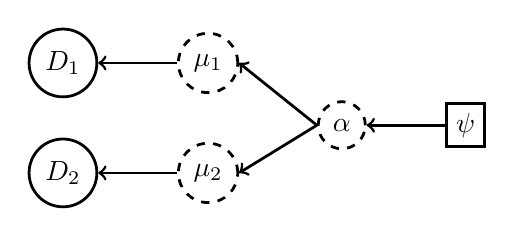
\begin{tikzpicture}
\node[circle, draw, line width=1pt] (D1) {$D_1$};
\node[circle, draw, below=0.5cm of D1, line width=1pt] (D2) {$D_2$};
\node[circle, dashed, draw, right=1cm of D1, line width=1pt] (mu1) {$\mu_1$};
\node[circle, dashed, draw, right=1cm of D2, line width=1pt] (mu2) {$\mu_2$};
\node[circle, dashed, draw, below right=0.25cm and 3cm of D1, line width=1pt] (alpha) {$\alpha$};
\node[rectangle, draw, right=1cm of alpha, line width=1pt] (psi) {$\psi$};
\draw[->, line width=1pt] (mu1.west) -- (D1.east) {};
\draw[->, line width=1pt] (mu2.west) -- (D2.east) {};
\draw[->, line width=1pt] (alpha.west) -- (mu1.east) {};
\draw[->, line width=1pt] (alpha.west) -- (mu2.east) {};
\draw[->, line width=1pt] (psi.west) -- (alpha.east) {};
\end{tikzpicture}
\end{document}